\documentclass[conference]{IEEEtran}
\IEEEoverridecommandlockouts

\usepackage{cite}
\usepackage{amsmath,amssymb,amsfonts}
\usepackage{algorithmic}
\usepackage{graphicx}
\usepackage{textcomp}
\usepackage{xcolor}
\usepackage[utf8]{inputenc}
\usepackage{makecell}
\usepackage[spanish,mexico,english,activeacute]{babel}
\usepackage{float}
\usepackage{amsmath}
\usepackage{booktabs}
\usepackage{lscape}
\usepackage{longtable}

\def\BibTeX{{\rm B\kern-.05em{\sc i\kern-.025em b}\kern-.08em
    T\kern-.1667em\lower.7ex\hbox{E}\kern-.125emX}}
    
    \setlength{\intextsep}{1ex} % set space above and below in-line float
    \setlength{\intextsep}{-1ex} % remove extra space above and below in-line float

    
\begin{document}



\title{Aprendizaje de máquina para determinar el incumplimiento de pago en tarjetas de crédito
}
\author{\IEEEauthorblockN{Jose Alberto Arango Sánchez}
\IEEEauthorblockA{\textit{Ingeniería de Sistemas} \\
\textit{Universidad de Antioquia}\\
Medellín, Colombia \\
jose.arangos@udea.edu.co}
\and
\IEEEauthorblockN{Leon Dario Arango Amaya}
\IEEEauthorblockA{\textit{Ingeniería de Sistemas} \\
\textit{Universidad de Antioquia}\\
Medellín, Colombia \\
leon.arango@udea.edu.co}
}

\maketitle

\begin{abstract}
Este estudio tiene como objetivo realizar una comparación entre modelos clásicos del \textbf{Machine learning} como: KNN, SVM, RNA, Random Forest y Naïve Bayes, usados como clasificadores para determinar el incumplimiento de pago de una tarjeta de crédito. 
Los modelos que presentaron mejores medidas de desempeño, fueron: Random Forest y Maquina de Soporte Vectorial, seguido de la Red Neuronal Artificial. Sin embargo el modelo Naïve Bayes, tiene mejores valores en la sensibilidad, lo que indica que logra predecir mejor los incumplimientos de pago frente a los demás. Finalmente, con el objetivo de reducir la dimensionalidad se realiza un proceso de selección y extracción de características buscando optimizar los modelos con mejores resultados.
\end{abstract}

\hfill
 
\begin{IEEEkeywords}
Aprendizaje de máquina, modelos fenomenológicos,incumplimiento de pago, selección de características, extracción de características, machine learning
\end{IEEEkeywords}

\section{Resumen}
Este estudio tiene como objetivo realizar una comparación entre modelos clásicos del \textbf{Machine learning} como: KNN, SVM, RNA, Random Forest y Naïve Bayes, usados como clasificadores para determinar el incumplimiento de pago de una tarjeta de crédito. 
Los modelos que presentaron mejores medidas de desempeño, fueron: Random Forest y Maquina de Soporte Vectorial, seguido de la Red Neuronal Artificial. Sin embargo el modelo Naïve Bayes, tiene mejores valores en la sensibilidad, lo que indica que logra predecir mejor los incumplimientos de pago frente a los demás. Finalmente, con el objetivo de reducir la dimensionalidad se realiza un proceso de selección y extracción de características buscando optimizar los modelos con mejores resultados.

\section{Introducción}
El mundo moderno cada día es más sorprendente, los avances en tecnología son cada vez mejores y la dificultad de los retos que surgen crece de forma exponencial. En este documento, pretende abordar una problemática del sector bancario, la cual ha sido objeto de estudio durante los últimos años para múltiples investigadores; se trata del incumplimiento de pagos con tarjetas de crédito y para ello se utilizó un conjunto de datos que tuvo origen en Taiwan a mediados del 2005 [4]. El objetivo de este estudio es evaluar cinco algoritmos diferentes de aprendizaje automático, sacar métricas para cada uno de ellos y así poder determinar cual de éstos es mejor. Posteriormente se realizara un proceso de selección y extracción de características, con el fin de optimizar los mejores modelos y determinar cual de éstos realiza mejores predicciones, para resolver la problemática en cuestión. 

\section{Descripción del problema}

\subsection{El problema - Análisis de riesgo bancario}
Este es un problema supervisado de clasificación, y su propósito es determinar si una persona incumplirá con el pago de su tarjeta de crédito el próximo mes.

\subsection{Variables del problema}

El conjunto de datos utilizado consta de veintitrés características y una variable a predecir, las cuales se definen a continuación: 
\\
\begin{itemize}
    \item X1: Cupo del crédito otorgado en \$ NT Dollar. 
    \item X2: Genero (1: Male, 2: Female)
    \item X3: Nivel de educación ( 1:Postgrado, 2:Universidad, 3:Secundaria, 4:Otros)
    \item X4: Estado civil ( 1:Casado, 2:Soltero, 3:Otros)
    \item X5: Edad (años de la persona)
    \item X6-11: Historial de pago mes  mes en orden descendente.
        \begin{itemize}
            \item X6: Estado pagó SEPTIEMBRE de 2005.
            \item X11:Estado pagó ABRIL de 2005.
             \begin{itemize}
                \item -2: No se usó la tarjeta.
                \item -1: Pagó debidamente.
                \item  0: El cliente pagó el monto mínimo adeudado.
                \item  1:Retraso de 1 mes.
                \item  9:Retraso de 9 meses o mas.
             \end{itemize}
         \end{itemize}
    \item X12-17: Monto del estado de cuenta en de SEPTIEMBRE - ABRIL respectivamente en \$ NT Dollar.
    \begin{itemize}
            \item X12: Monto del estado de cuenta en de SEPTIEMBRE 2005.
            \item X17: Monto del estado de cuenta en de ABRIL 2005.
            \item Lo que se le debe al banco o si este es negativo es lo que el banco debe a la persona.
         \end{itemize}
    \item X18-23: Monto del pago anterior \$ NT Dollar.
        \begin{itemize}
            \item X18: Monto pagado en SEPTIEMBRE de 2005.
            \item X17: Monto pagado en ABRIL del 2005.
            \item Pago que se le realizo al banco.
         \end{itemize}
    \item Y: Incumplimiento de pago al siguiente mes (Si:1, No:0)\\
\end{itemize}
Es importante resaltar que el conjunto de datos no requiere imputación, ya que las muestras están completas. 

\section{Estado del arte}
Determinar si un cliente incumplirá en el pago de su tarjeta, Representa un problema de iteres para el sector bancario, debido a que la minimización de riesgos genera mayor esperanza de retorno del dinero. Por lo tanto es importante dar solución a este problema de una manera objetiva y precisa, aprovechando la información con la que se cuenta de los clientes. Información que ha sido empleada por múltiples investigadores para abordar este problema, usando algoritmos de \textit{\textbf{Machine Learning}} y obteniendo muy buenos resultados.

A continuación se presentan 4 artículos relevantes que abordan el problema mencionado anteriormente. estos emplean las misma base de datos usada en este artículo:
\subsection{The comparisons of data mining techniques for the predictive accuracy of probability of default of credit card clients }\label{AA} 
En este articulo se realiza \cite{articulo1} una comparación de 6 modelos clásicos del \textit{\textbf{Machine Learning}}, con el fin de determinar el incumplimiento del pago de una tarjeta el siguiente mes, por parte de un cliente asociado a un banco de Taiwán, con base en su información bancaria y personal. Además propone un método suavizado de clasificación, para determinar la probabilidad real del incumplimiento.
A continuación se presentan los modelos implementados en este artículo:
\hfill\\
\subsubsection{Modelos de aprendizaje automático implementados}
\begin{itemize}
\item K-nearest neighbor classifiers (KNN)
\item Logistic regression (LR)
\item Discriminant analysis (DA)
\item Naïve Bayesian classifier (NB)
\item Artificial neural networks (ANNs)
\item Classification trees (CTs)
\hfill\\
\end{itemize}
\subsubsection{Metodología de validación} \hfill\\
La metodología de validación empleada por estos investigadores fue bootstrapping \cite{boostrap}. Aunque no especifican la proporción de división del conjunto de datos.
\hfill\\
\subsubsection{Resultados obtenidos}\hfill\\
En la figura 1, se presenta una tabla con los resultados obtenidos para cada modelo, en la etapa de entrenamiento y validación:

\begin{center}
    \begin{figure}[H]
        \hfill
            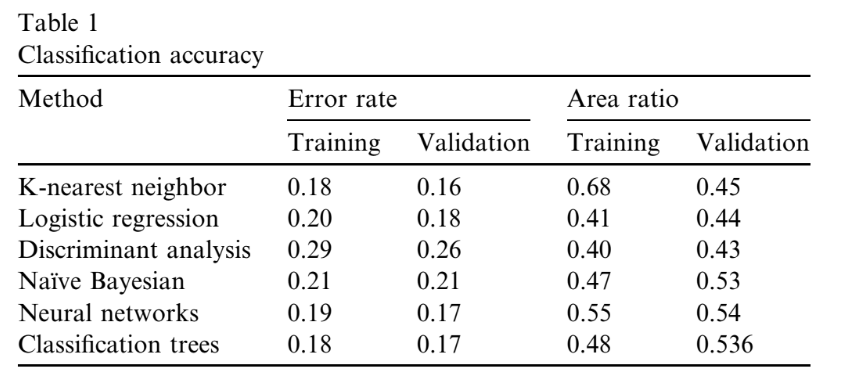
\includegraphics[width=8cm]{resultadosArticulo1.png}\hspace*{\fill}
    \caption{Resultados algoritmos evaluados}
    \label{fig:login}
    \end{figure}  
\end{center}

En este gráfico se aprecia un apartado llamado área ratio la cual esta dada por la siguiente expresión: \newline

\[
 \text{Relación de área} = \frac{\text{ACMCR}}{\text{AMCTCR}}
\]\newline
Donde ACMCR es el área entre la curva del modelo y la curva de referencia y AMCTCR es área entre la mejor curva teórica y la curva de referencia, como se observa en la figura 2.

Esta medida, es un criterio importante para la selección del mejor modelo, dado que un mayor valor representa una mayor similitud entre el modelo planteado y el teórico.
\begin{center}
    \begin{figure}[H]
        \hfill
            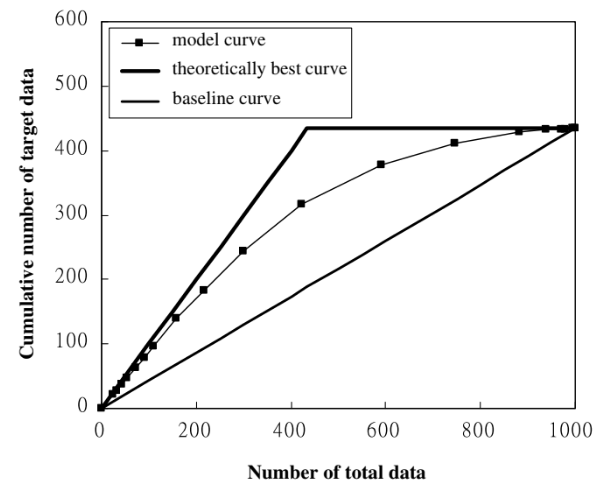
\includegraphics[width=8cm]{areaRatio.png}\hspace*{\fill}
    \caption{Relación de  área}
    \label{fig:login}
    \end{figure}  
\end{center}

Finalmente de la figura 1 y 2 se concluye que:
\begin{itemize}
\item El método KNN tiene un mejor desempeño en la fase de entrenamiento ya que cuenta con la tasa de error más baja y la relación de área más alta en esta misma fase. 
\item La red neuronal tiene mejor desempeño en la fase de validación, dado que su relación de área es la más alta entre todos los modelos, y su tasa de error es relativamente baja (0.17).
\end{itemize}
Finalmente los autores de este articulo recomiendan implementar redes neuronales artificiales, para calificar a los clientes.

\subsection{An experimental comparison of classification algorithms for imbalanced credit scoring data sets}

En este articulo se \cite{articulo2} compara varias técnicas de clasificación del \textbf{Machine learning}, para conjuntos de datos desequilibrados,  empleados en la calificación crediticia conocido comúnmente como \textbf{Scoring}.
Además de utilizar técnicas de clasificación tradicionales, como la regresión logística, las redes neuronales y los árboles de decisión, este artículo explora el \textbf{gradient boosting}, máquina de vector de soporte de mínimos cuadrados y random forests para la predicción del incumplimiento de pago.

Los criterios de rendimiento elegidos en este artículo para medir el efecto del desbalanceo en los diferentes modelos son: el área bajo la curva (AUC), la estadística de Friedman y las pruebas post hoc de Nemenyi.
A continuación se presentan los modelos implementados en este artículo:
\subsubsection{Modelos de aprendizaje automático implementados}
\begin{itemize}
\item Logistic regression
\item Linear and quadratic discriminant analysis
\item Neural networks (Multi-layer perceptron)
\item Least square support vector machines (LS-SVMs)
\item C4.5. decision trees
\item k-NN (memory based reasoning)
\item Random forests
\item Gradient boosting
\end{itemize}
\hfill\\
\subsubsection{Metodología de validación}\hfill\\
La metodología de validación empleada fue Bootstrapping, con una proporción de 
$\frac{2}{3}$ del \textit{dataset} para el entrenamiento y $\frac{1}{3}$ para las pruebas. 
\hfill\\
\subsubsection{Resultados obtenidos}
\begin{itemize}
\item Random forests y gradiente boosting fueron los de mejor resultado debido a que tiene un AUC mayor.
\item Decision tree,  quadratic discriminant analysis y KNN obtienen los peores resultados.
\item Las técnicas de sobremuestreo tiene mejor resultado que las técnicas de submuestreo.
\item El Random forests funciona sorprendentemente bien dado un gran desequilibrio de clases.
\end{itemize}
\subsection{Application of machine learning algorithms in credit card default payment prediction}

En este trabajo se realiza una comparación de ocho modelos diferentes de los cuales sacan la precisión, sensibilidad y especificidad como métricas para evaluar el rendimiento. Además con base en estos resultados  obtener el mejor modelo. \\

\subsubsection{Modelos de aprendizaje automático implementados}
\begin{itemize}
\item Naïve Bayes
\item K-nearest neighbor
\item support vector machine
\item Logistic regression
\item Classification trees
\item Bagging
\item Boosting
\item Voting
\end{itemize}
\hfill
\subsubsection{Metodología de validación}\hfill

La metodología de validación utilizada fue validación cruzada con diez k-fold
\\

\subsubsection{Resultados obtenidos}\hfill

Según el estudio de  Husejinovic, Keco y Masetić [6], se determinó que el mejor modelo es la regresión logística con una eficiencia de 0.820, seguido de la máquina de soporte vectorial con 0.819 Figura ~\ref{fig:Accuracy_4}
\\

\begin{center}
    \begin{figure}[h]
        \hfill
            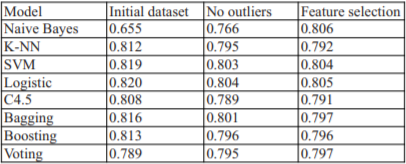
\includegraphics[width=8cm]{Accuracy_4.png}\hspace*{\fill}
    \caption{Eficiencia de los modelos}
    \label{fig:Accuracy_4}
    \end{figure}
\end{center}

\subsection{Credit default mining using combined machine learning and heuristic approach}

La investigación realizada por Islam, Eberle y Ghafoor [7], buscaba encontrar la solución al problema desde dos enfoques diferentes: uno heurístico y a través del aprendizaje de Máquina. Los investigadores concluyen que el aprendizaje de máquina es mejor por aproximadamente 2\% de exactitud. Para determinar esto, utilizan cinco modelos diferentes: 
\begin{itemize}
\item Random Forest
\item Naïve Bayes
\item Gradient Boosting
\item K-nearest neighbor
\item Extremly Randomized Trees
\end{itemize}
\hfill
\subsubsection{Metodología de validación}\hfill\\
La metodología de validación utilizada fue validación cruzada con diez k-fold
\hfill\\
\subsubsection{Resultados obtenidos}\hfill\\
Según los investigadores, los mejores modelos para tratar este problema son árboles extremadamente aleatorios con una eficiencia de 0.958 y árboles aleatorios con 0.944 Figura ~\ref{fig:Accuracy_3}\\ 

\begin{center}
    \begin{figure}[H]
        \hfill
            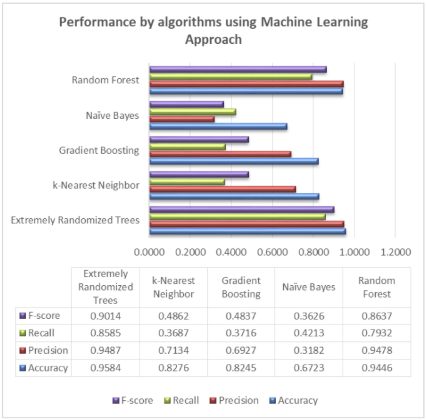
\includegraphics[width=8cm]{Accuracy_3.png}\hspace*{\fill}
    \caption{Eficiencia de los modelos}
    \label{fig:Accuracy_3}
    \end{figure}  
\end{center}

 Los resultados obtenidos por estos investigadores son buenos, pero no es posible saber cómo llegaron a ellos, ya que hicieron poco énfasis en los procedimientos.

\section{Experimentos}
  Para los siguientes experimentos se empleó la base de datos: \textit{default of credit card clients Data Set} \cite{bd}. Esta base de datos cuenta con la información crediticia de 30.000 clientes, descrita por  23 características (ver sección 2B). Es importante especificar que la base de datos no contiene datos faltantes.

El problema se abordó como un modelo de clasificación biclase, en el cual las clases corresponden a: 

\begin{itemize}
\item 0: La persona no incumplirá en el pago de su tarjeta en el siguiente mes.
\item 1: La persona incumplirá en el pago de su tarjeta en el siguiente mes.
\end{itemize}
Se tiene un desbalanceo entre clases el cual se puede visualizar en la figura ~\ref{fig:frecuenciaClases}
\begin{center}
    \begin{figure}[H]
        \hfill
            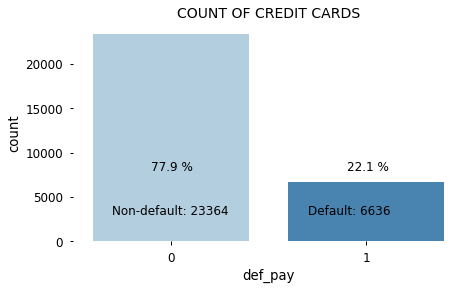
\includegraphics[width=8cm]{desbalnaceo.png}\hspace*{\fill}
    \caption{Frecuencia de clases}
    \label{fig:frecuenciaClases}
    \end{figure}  
\end{center}
Además, las características se encuentran en diferentes escalas como se logra apreciar en la figura ~\ref{fig:escalaVariables}. Por lo tanto se realizo una normalización de todas estas con el criterio \textit{Z-SCORE}. 
\begin{center}
    \begin{figure}[H]
        \hfill
            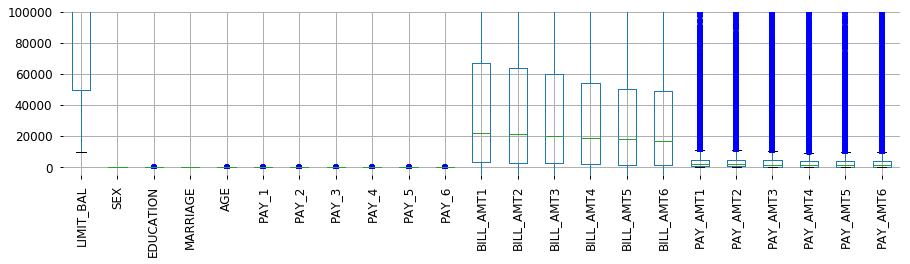
\includegraphics[width=8cm]{escala.png}\hspace*{\fill}
    \caption{Escala de variables}
    \label{fig:escalaVariables}
    \end{figure}  
\end{center}
La normalización ocasiona que la distribución tenga media 0 y desviación estándar 1, como se visualiza en la figura ~\ref{fig:violinPlot} mediante el Violin plot.

\begin{center}
    \begin{figure}[H]
        \hfill
            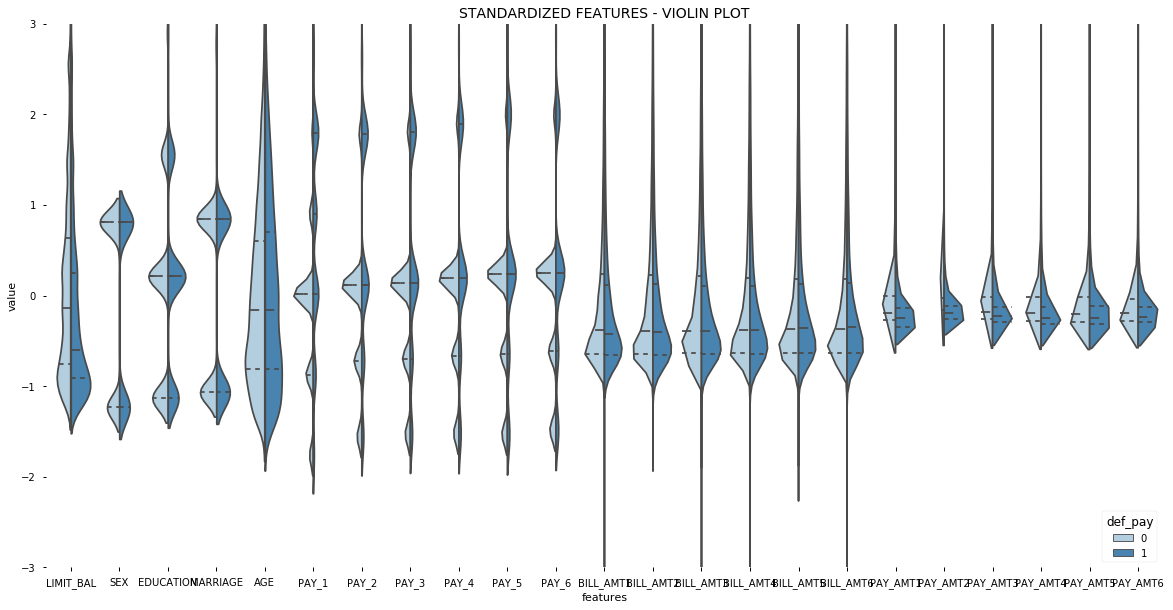
\includegraphics[width=8cm]{violin.png}\hspace*{\fill}
    \caption{Violin Plot}
    \label{fig:violinPlot}
    \end{figure}  
\end{center}
Finalmente para atacar el problema de desbalanceo de clases, se empleo validación cruzada estratificada con 10 \textit{folds} como lo sugiere el articulo 3. El conjunto de datos se dividió en tres partes, un subconjunto de entrenamiento y de validación que equivale al \text{80\%} del total de muestras y uno de pruebas con el 20\%. Esto con el fin de determinar el comportamiento de los modelos entrenados frente a muestras que no conozcan, evaluando su capacidad de generalización.
A continuación se presentaran los resultados obtenidos en 5 modelos diferentes:

\subsection{Naïve Bayes}
En este modelo, se utilizaron los parámetros por defecto, incluidos en la librería sklearn \cite{sklearnGaussian}. Obteniendo un \textit{Acurracy} del 67\%. Otras medidas de desempeño utilizadas fueron: sensibilidad, especificidad, eficiencia y precisión las cuales se obtuvieron a partir de la figura ~\ref{fig:confusionMatrizGNB} o bien llamada matriz de confusión y se aprecian en la tabla  ~\ref{tab:medidasGNB}
\begin{center}
    \begin{figure}[H]
        \hfill
     \centerline{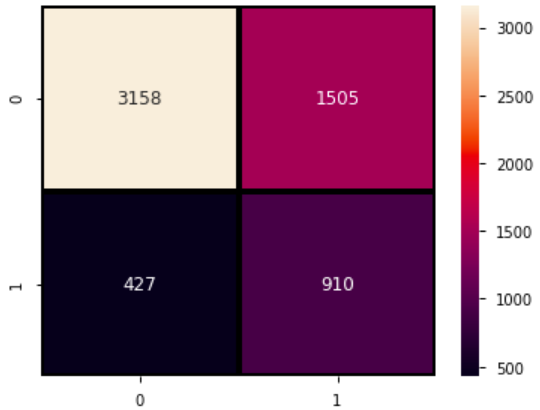
\includegraphics[width=8cm]{matrixConfusionGNB.png}}
    \caption{Matriz de confusión del modelo Naïve Bayes}
    \label{fig:confusionMatrizGNB}
    \end{figure}  
\end{center}
\begin{table}[H]
\centering
\begin{tabular}{|l|l|l|l|}
\hline
Sensibilidad & Especificidad & \multicolumn{1}{r|}{Eficiencia} & Precisión \\ \hline
0,68         & 0,68          & 0,68                            & 0,38      \\ \hline
\end{tabular}
\caption{Medidas de desempeño del modelo Naïve Bayes}
\label{tab:medidasGNB}
\end{table}
Durante la fase de entrenamiento se logró una eficiencia de 0.6749 con un intervalo de confianza de +/- 0.0362. Mientras que en la fase de validación, una eficiencia de 0.6742 con un intervalo de confianza de +/-  0.0372. Siendo estas unas medidas de desempeño no tan buenas, sin embargo este modelo clasifica mucho mejor las muestras de la clase 1(personas que incumplirá en el pago de su tarjeta en el siguiente mes), que los otros modelos vistos, con un porcentaje del 68\% de acierto, el cual es dado por la sensibilidad.

Finalmente a través de la figura ~\ref{fig:rocGNB}, llamada curva ROC, la cual es una representación gráfica de la sensibilidad frente a la especificidad, para un sistema clasificador binario. llegamos a la conclusión de que este modelo se comporta de una manera muy regular, al momento de realizar la clasificación.
\begin{center}
    \begin{figure}[H]
        \hfill
     \centerline{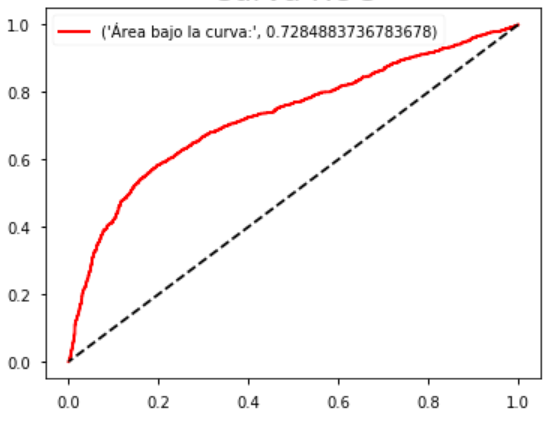
\includegraphics[width=8cm]{ROCGNB.png}}
    \caption{Curva ROC modelo Naïve Bayes }
    \label{fig:rocGNB}
    \end{figure}  
\end{center}
\subsection{K vecinos mas cercanos (KNN)}
En este modelo se realizaron las siguiente combinaciones de parámetros que se pueden apreciar en la tabla~\ref{tab:parametrosKNN}
\newline
\begin{table}[H]
\centering
\begin{tabular}{|l|l|}
\hline
Parametro    & Valores              \\ \hline
n\_neighbors & 10,20,30,40,50       \\ \hline
metric    & minkowski, euclidean, manhattan    \\ \hline
\end{tabular}
\caption{Combinación de parámetros empleada para el modelo kNN}
\label{tab:parametrosKNN}
\end{table}
La mejor combinación de parámetros encontrada fue: metric: minkowski y n\_neighbors: 11, la cual obtuvo un \textit{Acurracy} del 81\%.
Durante la fase de entrenamiento se logró una eficiencia de 0.8271 con un intervalo de confianza de +/- 0.0010. Mientras que en la fase de validación, una eficiencia de 0.8058 con un intervalo de confianza de +/- 0.0054. Siendo estos unos resultados aceptables en comparación con el modelo Naïve Bayes.
Como se han venido presentado los resultados en modelos previos, la figura ~\ref{fig:matrixRDF}  y figura ~\ref{fig:rocRDF} son la matriz de confusión y la curva ROC para este modelo.

\begin{center}
    \begin{figure}[H]
        \hfill
     \centerline{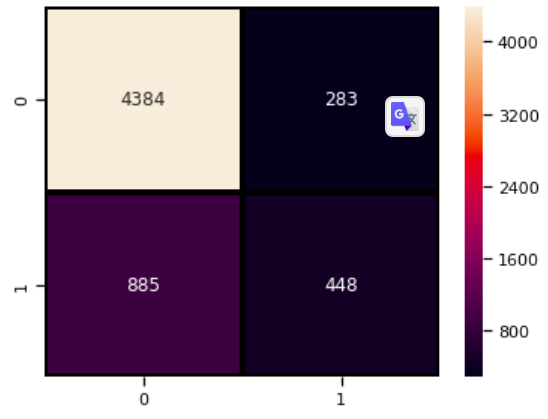
\includegraphics[width=8cm]{MatrixKNN.png}}
    \caption{Matriz de confusión del modelo KNN }
    \label{fig:matrixKNN}
    \end{figure}  
\end{center}

\begin{center}
    \begin{figure}[H]
        \hfill
     \centerline{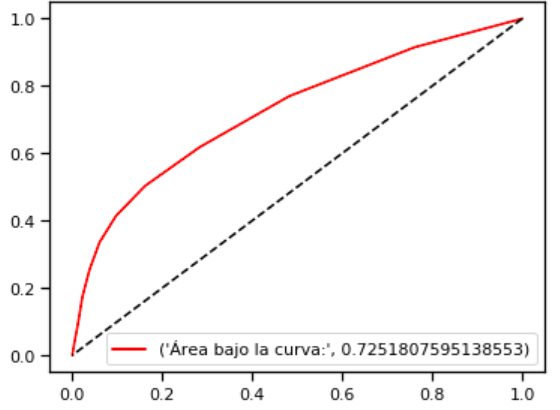
\includegraphics[width=8cm]{ROCKNN.png}}
    \caption{Curva ROC modelo KNN }
    \label{fig:rocKNN}
    \end{figure}  
\end{center}
De la matriz de confusión, se obtienen las medidas de desempeño de la tabla  ~\ref{tab:medidasGknn}  
\newline
\begin{table}[H]
\centering
\begin{tabular}{|l|l|l|l|}
\hline
Sensibilidad & Especificidad & \multicolumn{1}{r|}{Eficiencia} & Precisión \\ \hline
0,34         & 0,94          & 0,81                            & 0,61      \\ \hline
\end{tabular}
\caption{Medidas de desempeño del modelo KNN}
\label{tab:medidasGknn}
\end{table}

Finalmente se concluye que este modelo:
\begin{itemize}
\item El 81\% de las muestras predichas fueron correctamente clasificadas.
\item No presenta sobre ajuste, ya que el error en entrenamiento no es cercano a cero y el de validación no es muy grande.
\item Los errores son similares , sin embargo se tiene mayor error en la fase de validación que en entrenamiento, como es de esperar según la teoría.
\item Según la sensibilidad solo el 34\% de las muestras de la clase 1 (personas que incumplirá en el pago de su tarjeta en el siguiente mes), están siendo correctamente clasificadas.
\item El modelo esta clasificando el 94\% de las muestras de la clase 0 (persona que no incumplirá en el pago de su tarjeta en el siguiente mes), correctamente.
\item Dado los valores de sensibilidad y especificidad, el modelo clasifica bien muestras de la clase 0 (la clase mayoritaria), caso contrario las muestras clase 1 (clase minoritaria). Por lo tanto se debe implementar otra manera de abordar el desabalanceo de clases al momento de entrenar este modelo.
\item El área bajo la curva de este modelo es muy regular, incluso mas baja que el modelo Naïve Bayes por lo tanto, el modelo  tiene capacidad de separación de clases pero no es muy bueno.
\end{itemize}
\subsection{Redes Neuronales Artificiales (RNA)}
En este modelo se realizaron las siguiente combinaciones de parámetros la cual se puede apreciar en la tabla~\ref{tab:parametrosGNA}\hfill\\

\begin{table}[H]
\centering
\begin{tabular}{|l|l|}
\hline
Parametro    & Valores              \\ \hline
solver & adam       \\ \hline
max\_iter    & 300   \\ \hline
alpha    &  0.1  , 0.01 , 0.001  \\ \hline
hidden\_layer\_sizes    & 300   \\ \hline
activation    & logistic, tanh   \\ \hline
\end{tabular}
\caption{Combinación de parámetros empleada para el modelo de Redes Neuronales Artificiales}
\label{tab:parametrosGNA}
\end{table}
La mejor combinación de parámetros encontrada fue: Red neuronal artificial con función de activación logística, alpha = 0.01, numero de neuronas por capa = 72, máximo numero de iteraciones = 300 y el método para la optimización de los pesos = adam, que obtuvo un \textit{Acurracy} del 82\%.
Durante la fase de entrenamiento se logró una eficiencia de 0.8228 con un intervalo de confianza de +/-  0.0010. Mientras que en la fase de validación, una eficiencia de 0.8197 con un intervalo de confianza de +/- 0.0044.
Como se han venido presentado los resultados en modelos previos, la figura ~\ref{fig:matrixGNA}  y figura ~\ref{fig:rocRNA} son la matriz de confusión y la curva ROC respectivamente, para este modelo.
\begin{center}
    \begin{figure}[h]
        \hfill
     \centerline{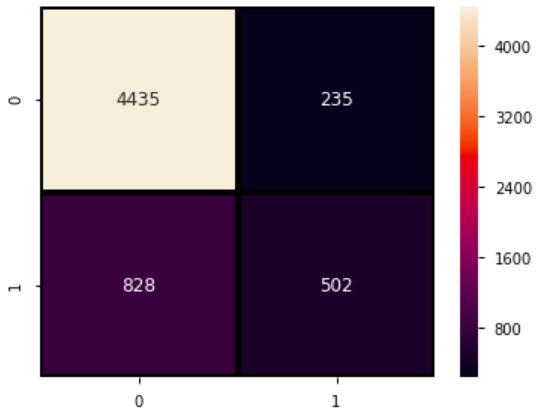
\includegraphics[width=8cm]{MatrixGNA.png}}
    \caption{Matriz de confusión del modelo de Redes Neuronales Artificiales}
    \label{fig:matrixGNA}
    \end{figure}  
\end{center}

\begin{center}
    \begin{figure}[h]
        \hfill
     \centerline{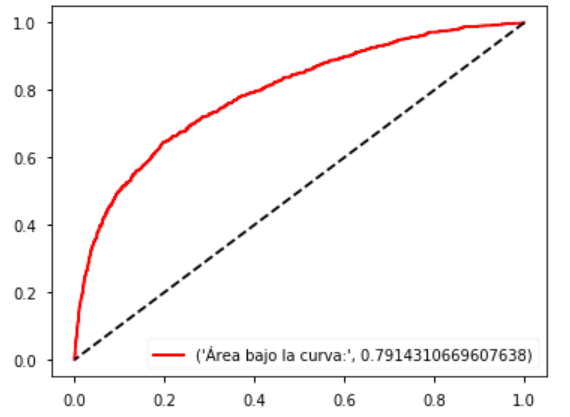
\includegraphics[width=8cm]{ROCGNA.png}}
    \caption{Curva ROC modelo de Redes Neuronales Artificiales }
    \label{fig:rocRNA}
    \end{figure}  
\end{center}
El resultado de las medidas de desempeño, expresado en la tabla ~\ref{tab:medidasRNA} fue:
\newline
\begin{table}[H]
\centering
\begin{tabular}{|l|l|l|l|}
\hline
Sensibilidad & Especificidad & \multicolumn{1}{r|}{Eficiencia} & Precisión \\ \hline
0,38         & 0,95          & 0,82                            & 0,68      \\ \hline
\end{tabular}
\caption{Medidas de desempeño del modelo de Redes Neuronales Artificiales}
\label{tab:medidasRNA}
\end{table}
Finalmente se concluye que en este modelo:
\begin{itemize}
\item El 82\% de las muestras fueron clasificadas correctamente, lo cual es un resultado muy bueno en comparación con los otros modelos.
\item Al igual que el modelo KNN, este modelo no presenta sobreajuste. 
\item No se presenta subajuste, ya que para cumplir dicha condición el error durante el entrenamiento y validación debe ser elevado y similar para ambos casos; condición que no cumple este modelo.
\item Este modelo presenta las misma falencias que el modelo KNN, respecto a la clasificación de muestras de la clase 1,sin embargo es un 4\% mejor que este.
\item 68\% de precisión indica que hay una mediana proximidad entre los valores obtenidos en mediciones repetidas.
\item El área bajo la curva de este modelo es mejor, que la de los modelo Naïve Bayes y KNN. Llegando casi al 0.8 valor levemente cercado a 1, que es el valor ideal. Por lo tanto, el modelo  tiene una mayor capacidad de separación de clases respecto a los otros.
\end{itemize}
\subsection{Random Forest}
En este modelo se realizaron las siguiente combinaciones de parámetros que se pueden apreciar en la tabla~\ref{tab:parametrosRDF}
\hfill
\\ 
\begin{table}[H]
\centering
\begin{tabular}{|l|l|}
\hline
Parametro    & Valores              \\ \hline
max\_features & 10,20,30,40,50       \\ \hline
max\_features & 1,2,3,4,5            \\ \hline
max\_depth    & 1,2,3,4,5,8,10,15,20 \\ \hline
criterion    & gini, entropy    \\ \hline
\end{tabular}
\caption{Combinación de parámetros para el modelo Random Forest}
\label{tab:parametrosRDF}
\end{table}
La mejor combinación de parámetros encontrada fue: criterion: entropy, max\_depth: 8, max\_features: 5 y n\_estimators: 50, la cual obtuvo un \textbf{Acurracy} del 83\%

Durante la fase de entrenamiento se logró una eficiencia de 0.9514 con un intervalo de confianza de +/- 0.0012. Mientras que en la fase de validación, una eficiencia de 0.8263  con un intervalo de confianza de +/- 0.0051. Siendo estos unos resultados buenos en comparación a los del modelo Naïve Bayes y el KNN.
Como se han venido presentado los resultados en modelos previos, la figura ~\ref{fig:matrixRDF}  y figura ~\ref{fig:rocRDF} corresponden a la matriz de confusión y la curva ROC respectivamente, para este modelo.

\begin{center}
    \begin{figure}[H]
        \hfill
     \centerline{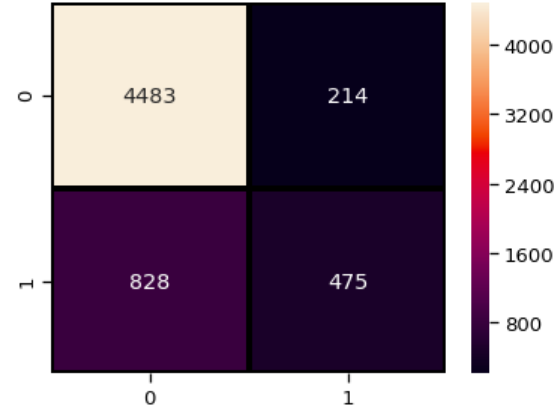
\includegraphics[width=8cm]{matrixRDF.png}}
    \caption{Matriz de confusión del modelo Random Forest }
    \label{fig:matrixRDF}
    \end{figure}  
\end{center}

\begin{center}
    \begin{figure}[H]
        \hfill
     \centerline{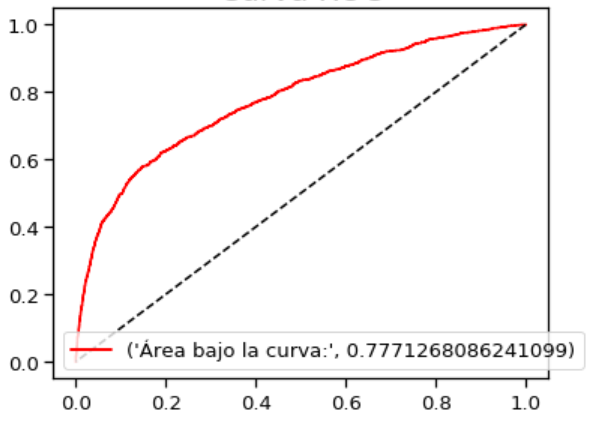
\includegraphics[width=8cm]{ROCRDF.png}}
    \caption{Curva ROC del modelo Random Forest }
    \label{fig:rocRDF}
    \end{figure}  
\end{center}

El resultado de las medidas de desempeño, son los presentados en la tabla ~\ref{tab:medidasRDF}:
\newline
\begin{table}[H]
\centering
\begin{tabular}{|l|l|l|l|}
\hline
Sensibilidad & Especificidad & \multicolumn{1}{r|}{Eficiencia} & Precisión \\ \hline
0,36         & 0,95          & 0,83                            & 0,69      \\ \hline
\end{tabular}\hfill\\
\caption{Medidas de desempeño del modelo Random Forest}
\label{tab:medidasRDF}
\end{table}
Finalmente se concluye que en este modelo:
\begin{itemize}
\item El 83\% de las muestras fueron clasificadas correctamente, lo cual es un resultado bueno en comparación a los otros modelos.
\item Al igual que el modelo KNN, este modelo no presenta sobreajuste, sin embargo dada la alta eficiencia (95\%) durante el entrenamiento se puede observar indicios de memorización de muestras.
\item Este modelo presenta las misma falencias que el modelo KNN y la RNA, respecto a la clasificación de muestras de la clase 1.
\item 69\% de precisión indica que hay una mediana proximidad entre los valores obtenidos en mediciones repetidas, lo cual es un aumento leve respecto a la red neuronal artificial.
\item El área bajo la curva de este modelo es mejor que el modelo KNN, pero menor que la RNA, cercano a 1 que es el valor de referencia. Por lo tanto, el modelo  tiene una buena capacidad de separación.
\item El costo computacional de este modelo es mucho menor que el empleado por la RNA, además obtiene resultados muy similares.
\end{itemize}

\subsection{Maquinas de Soporte Vectorial}\hfill
En este modelo se realizaron las siguiente combinaciones de parámetros la cual se puede apreciar en la tabla~\ref{tab:parametrosSVM} \hfill\\
\begin{table}[H]
\centering
\begin{tabular}{|l|l|}
\hline
Parámetro    & Valores          \\ 
C & 0.001, 0.01, 0.1, 1,        \\ 
gamma    & 0.001, 0.01, 0.1, 1  \\ 
alpha    &  0.1  , 0.01 , 0.001  \\ 
kernel    & rbf,linear   \\ \hline
\end{tabular}\hfill
\caption{Combinación de parámetros para la Maquinas de Soporte Vectorial}
\label{tab:parametrosSVM}\hfill\\
\end{table} 
La mejor combinación de parámetros encontrada fue: Maquina de soporte vectorial con C = 1, gamma = 0.1 y kernel rbf, obteniendo un \textbf{Acurracy} del 83\%.
Durante la fase de entrenamiento se logró una eficiencia de 0.8205 con un intervalo de confianza de +/- 0.000800. Mientras que en la fase de validación, una eficiencia de 0.832  con un intervalo de confianza de +/-  0.00479. Siendo estos unos buenos resultados.
Como se han venido presentado los resultados en modelos previos, la figura ~\ref{fig:matrixSVM}  y figura ~\ref{fig:rocSVM} representan la matriz de confusión y la curva ROC respectivamente para este modelo.
\begin{center}
    \begin{figure}[H]
        \hfill
     \centerline{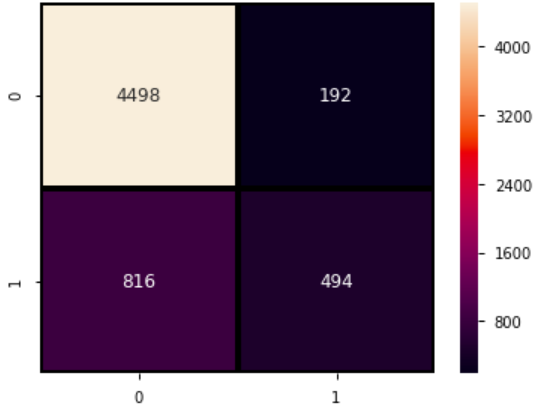
\includegraphics[width=8cm]{MatrixSVM.png}}
    \caption{Matriz de confusión del modelo de las Maquinas de Soporte Vectorial}
    \label{fig:matrixSVM}
    \end{figure}  
\end{center}

\begin{center}
    \begin{figure}[h]
        \hfill
     \centerline{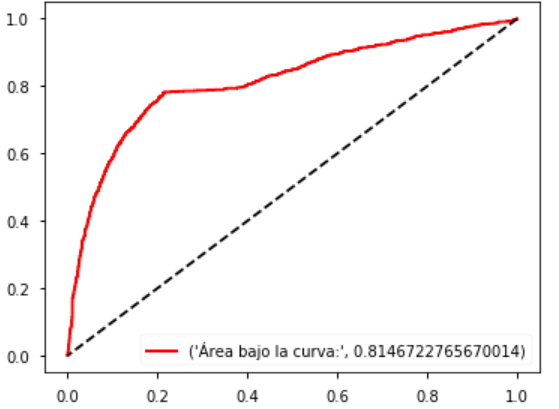
\includegraphics[width=8cm]{ROCSVM.png}}
    \caption{Curva ROC modelo de las Maquinas de Soporte Vectorial}
    \label{fig:rocSVM}
    \end{figure}  
\end{center}
El resultado de las medidas de desempeño, se expresa en la tabla ~\ref{tab:medidasRNA}: 
\newline
\begin{table}[h]
\centering
\begin{tabular}{|l|l|l|l|}
\hline
Sensibilidad & Especificidad & \multicolumn{1}{r|}{Eficiencia} & Precisión \\ \hline
0,38         & 0,96          & 0,83                            & 0,72      \\ \hline
\end{tabular}
\caption{Medidas de desempeño del modelo de Maquinas de Soporte Vectorial}
\label{tab:medidasRNA}
\end{table}

Finalmente se concluye que este modelo:
\begin{itemize}
\item Tiene la mayor área bajo la curva (0.81) de todos los modelos mencionados anteriormente. Por lo tanto, tiene una mayor capacidad de separación entre clases.
\item Tiene las mejores medidas desempeño, en comparación a los modelos anteriormente vistos. estas medidas se expresan en la tabla ~\ref{tab:medidasRNA}.
\item Es igual de bueno que el Random Forest para clasificar muestras correctamente, con una certeza del 83\%
\item Presenta las misma dificultades que el KNN, Random Forest Y RNA para la clasificación de muestra de la clase 1.
\end{itemize}

\section{Análisis de características}
Trabajar con las 23 características al tiempo, implica un costo computacional elevado. No obstante puede presentarse que algunas características no aporte mucha información a los modelos, siendo redundantes.  También es importante cumplir el principio de parsimonia, el cual consiste en que el modelo mas simple, será siempre el escogido como solución. Por lo tanto es importante considerar la reducción de dimensionalidad, es decir, trabajar con menos variables.

Para lograr este fin, se plantearon dos métodos: Realizando selección y extracción de características. Sin embargo, para poder emplear estas estrategias se debe realizar una primera estimación de la cantidad de variables a eliminar, para el caso de selección; y una cantidad de componentes a seleccionar, para el caso de extracción. Dicha estimación se puede obtener de una manera experimental, mediante el análisis individual de cada una de las características, a partir de medidas de correlación y del índice de Fisher.

Empleando la matriz de correlación de la figura ~\ref{fig:matrizCorrelation} y solo analizando la correlación entre variables, ya que las relaciones con la variable a predecir, no tiene ninguna interpretación valida en problemas de clasificación. Se puede determinar las características candidatas a ser eliminadas.
\begin{center}
    \begin{figure}[H]
        \hfill
     \centerline{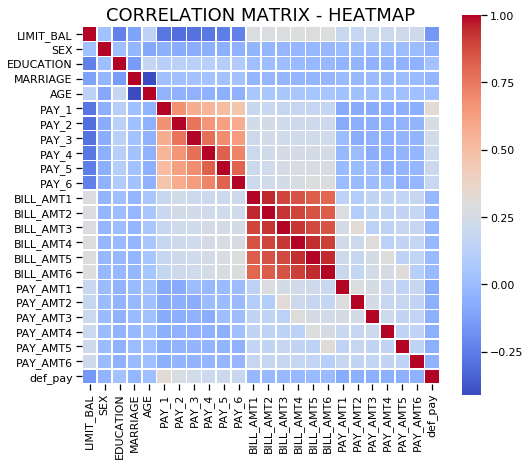
\includegraphics[width=8cm]{correlacion.png}}
    \caption{Matriz de correlación }
    \label{fig:matrizCorrelation}
    \end{figure}  
\end{center}
Mayor intensidad de color rojo, entre las parejas de variables a evaluar, implica una correlación fuerte entre ellas. De la figura ~\ref{fig:matrizCorrelation} se logra apreciar que dicha condición es cumplida por las variables: BILL\_AMT1, BILL\_AMT2, BILL\_AMT3, BILL\_AMT4, BILL\_AMT5, BILL\_AMT5, en mayor proporción y en menor medida por las variables: PAY\_1, PAY\_2, PAY\_3, PAY\_4, PAY\_5, PAY\_6, ya que estas presentan una menor intensidad. Por lo tanto las 12 variables mencionadas anteriormente son las cándidas a ser eliminadas.

Empleando el índice discriminante de \textbf{Fisher} se obtiene los siguientes resultados:
\begin{center}
    \begin{figure}[H]
        \hfill
     \centerline{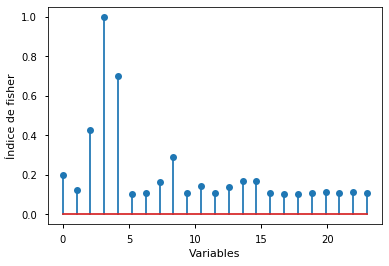
\includegraphics[width=8cm]{fisher.png}}
    \caption{Índices de Fisher}
    \label{fig:indexFisher}
    \end{figure}  
\end{center}
En la gráfica ~\ref{fig:indexFisher}, se encuentran los índices de Fisher normalizados, para cada uno de las variables. Solo se conservarán aquellas variables cuyo índice de Fisher sea mayor a 0.5, ya que tienen un mayor poder discriminante. Por lo tanto las únicas variables a conservar para el entrenamiento son: EDUCATION, MARRIAGE y AGE.

Finalmente, por la matriz de correlación existen 12 variables candidatas a eliminar y por el índice de Fisher 20. Es importante aclarar que una de la suposición del índice de Fisher, es que las variables de entrada son independientes entre ellas.

\section{Selección de características}
Para emplear la selección de características, se debe definir como parámetro el numero de características a seleccionar. Dicho valor se obtuvo con base en la cantidad de variables a eliminar, arrojada por la matriz de correlación. Se empleó una función tipo \textbf{Wrapper}, con los tres mejores modelos obtenidos en la sección de experimentos, iterando de 10 a 20 variables de dos en dos y usando selección secuencial hacia adelante y hacia atrás.
A continuación se presentan los resultados alcanzados por cada modelo:
\subsection{Random Forest Classifier}\hfill
\begin{table}[h]
\centering
\begin{tabular}{lllll}
\hline
\multicolumn{5}{c}{\textbf{Random Forest Classifier}} \\ \hline
N & Forward & Error V & IC (std) & Eficiencia V \\ \hline
10 & TRUE & 0.1652 & 0.00090 & 83.45\% \\
13 & TRUE & 0.1648 & 0.00072 & 83.42\% \\
15 & TRUE & 0.1620 & 0.00083 & 83.73\% \\
18 & TRUE & 0.1619 & 0.00123 & 83.72\% \\
20 & TRUE & 0.1607 & 0.00100 & 83.76\% \\
10 & FALSE & 0.1640 & 0.00074 & 83.69\% \\
13 & FALSE & 0.1636 & 0.00080 & 83.67\% \\
15 & FALSE & 0.1617 & 0.00090 & 83.80\% \\
18 & FALSE & 0.1618 & 0.00082 & 83.79\% \\
20 & FALSE & 0.1605 & 0.00091 & 83.97\% \\ \hline
\end{tabular}
\end{table}\hfill
\newline
\newline
El mejor resultado obtenidos, dada su eficiencia en la fase de validación es:
\begin{itemize}
\item Random Forest con 20 características, en el siguiente orden de importancia:

LIMIT\_BAL, SEX, AGE, PAY\_0, PAY\_2, PAY\_3, PAY\_4, PAY\_5, PAY\_6, BILL\_AMT1, BILL\_AMT2, BILL\_AMT3, BILL\_AMT4, BILL\_AMT5, BILL\_AMT6, PAY\_AMT2, PAY\_AMT3, PAY\_AMT4, PAY\_AMT5, PAY\_AMT6.

\end{itemize}

\subsection{RNA Classifier}\hfill

\begin{table}[H]
\centering
\begin{tabular}{lllll}
\hline
\multicolumn{5}{c}{\textbf{RNA Classifier}} \\ \hline
N & Forward & Error V & IC (std) & Eficiencia V \\ \hline
10 & TRUE & 0.1774 & 0.00132 & 82.19\% \\
13 & TRUE & 0.1788 & 0.00072 & 82.12\% \\
15 & TRUE & 0.1755 & 0.00095 & 82.37\% \\
18 & TRUE & 0.1749 & 0.00060 & 82.39\% \\
20 & TRUE & 0.1745 & 0.00096 & 82.45\% \\
10 & FALSE & 0.1767 & 0.00088 & 82.25\% \\
13 & FALSE & 0.1760 & 0.00088 & 82.30\% \\
15 & FALSE & 0.1758 & 0.00053 & 82.38\% \\
18 & FALSE & 0.1748 & 0.00080 & 82.39\% \\
20 & FALSE & 0.1741 & 0.00099 & 82.44\% \\ \hline
\end{tabular}
\end{table}\hfill


El mejor resultado obtenidos, dada su eficiencia en la fase de validación es:
\begin{itemize}
\item Red neuronal artificial con 20 características, en el siguiente orden de importancia:

LIMIT\_BAL, SEX, EDUCATION, MARRIAGE, AGE, PAY\_0, PAY\_2, PAY\_4, PAY\_5, PAY\_6, BILL\_AMT1, BILL\_AMT2, BILL\_AMT3, BILL\_AMT5, BILL\_AMT6, PAY\_AMT1, PAY\_AMT2, PAY\_AMT4, PAY\_AMT5, PAY\_AMT6

\end{itemize}


\subsection{SVM Classifier}\hfill

\begin{table}[H]
\centering
\begin{tabular}{lllll}
\hline
\multicolumn{5}{c}{\textbf{SVM Classifier}} \\ \hline
N & Forward & Error V & IC (std) & Eficiencia V \\ \hline
10 & TRUE & 0.1724 & 0.00080 & 82.81\% \\
13 & TRUE & 0.1706 & 0.00076 & 82.98\% \\
15 & TRUE & 0.1691 & 0.00070 & 83.17\% \\
18 & TRUE & 0.1674 & 0.00078 & 83.25\% \\
10 & FALSE & 0.1722 & 0.00061 & 82.68\% \\
13 & FALSE & 0.1693 & 0.00056 & 83.03\% \\
15 & FALSE & 0.1678 & 0.00049 & 83.23\% \\
18 & FALSE & 0.1663 & 0.00055 & 83.32\% \\
20 & FALSE & 0.1655 & 0.00056 & 83.40\% \\ \hline
\end{tabular}
\end{table}\hfill

El mejor resultado obtenidos, dada su eficiencia en la fase de validación es:
\begin{itemize}
\item Maquina de soporte vectorial con 20 características, en el siguiente orden de importancia:

LIMIT\_BAL, SEX, EDUCATION, MARRIAGE, AGE, PAY\_0, PAY\_2, PAY\_3, PAY\_4, PAY\_5, PAY\_6, BILL\_AMT1, BILL\_AMT2, BILL\_AMT3, BILL\_AMT4, BILL\_AMT5, BILL\_AMT6, PAY\_AMT2, PAY\_AMT5, PAY\_AMT6

\end{itemize}
La gráfica ~\ref{fig:frecFeatures}, indica la frecuencia de cada característica, de los tres mejores modelos. En esta se ve claramente que del total de 22 características los 3 modelos consideran 16 de suma importancia.

\begin{center}
    \begin{figure}[H]
        \hfill
     \centerline{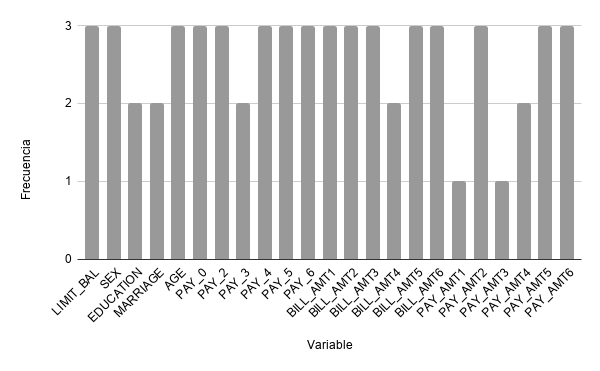
\includegraphics[width=8cm]{frecuencia.png}}
    \caption{Frecuencia de características mas relevantes}
    \label{fig:frecFeatures}
    \end{figure}  
\end{center}

\newline
Empleando 2 y 3 variables a seleccionar, las cuales fueron arrojadas por el análisis de Fisher. Se tiene los siguientes resultados por modelo:
Donde N: es el numero de características implementadas, Error V:es el error de validación, IC: es el intervalo de confianza y Eficiencia V: es la eficiencia durante la etapa de validación.

\subsection{Random Forest Classifier}\hfill
\begin{table}[H]
\centering
\begin{tabular}{lllll}
\hline
\multicolumn{5}{c}{\textbf{Random Forest Classifier}} \\ \hline
N & Forward & Error V & IC (std) & Eficiencia V \\ \hline
2 & TRUE & 0.17525 & 0.00050  &82.49\% \\
3 & TRUE & 0.17068 & 0.00029  &82.90 \% \\
2 & FALSE & 0.1772 & 0.00097 & 82.13 \% \\
3 & FALSE & 0.1733  & 0.00082 & 82.66 \% \\ \hline
\end{tabular}
\end{table}

\subsection{RNA Classifier}\hfill

\begin{table}[h]
\centering
\begin{tabular}{lllll}
\hline
\multicolumn{5}{c}{\textbf{RNA Classifier}} \\ \hline
N & Forward & Error V & IC (std) & Eficiencia V \\ \hline
2 & TRUE & 0.1800  & 0.0005  & 81.973\% \\
3 & TRUE & 0.1793 &  0.0006 & 81.982\% \\
2 & FALSE & &  & \% \\
3 & FALSE &  & & \% \\ \hline
\end{tabular}
\end{table}

\subsection{SVM Classifier}\hfill

\begin{table}[h]
\centering
\begin{tabular}{lllll}
\hline
\multicolumn{5}{c}{\textbf{SVM Classifier}} \\ \hline
N & Forward & Error V & IC (std) & Eficiencia V \\ \hline
2 & TRUE &  0.1789  & 0.0009  &82.25 \% \\
3 & TRUE &  0.1783 & 0.00089  & 82.32\% \\
2 & FALSE & 0.1790 & 0.0010 & 82.255 \% \\
3 & FALSE & 0.1783 & 0.0008 & 82.32\% \\ \hline
\end{tabular}
\end{table}

\section{Extracción de características}
La extracción de características es otro método para la reducción de la dimensionalidad. Este tiene como  objetivo. Conservar la mayor cantidad de información posible; realizando transformaciones de los datos originales a un nuevo conjunto de variables. Para este caso se empleo el análisis de componente principal (PCA), el cual parte del supuesto de que mayor variación implica más información.

A continuación se presentan los resultados registrados por este método, empleando como número de componentes, la cantidad de características usadas en la sección de selección.

\subsection{Random Forest Classifier}\hfill
\begin{table}[h]
\centering
\begin{tabular}{llll}
\hline
\multicolumn{4}{c}{\textbf{Random Forest Classifier}} \\ \hline
N & Error V & IC (std) & Eficiencia V \\ \hline
10 & 0.1964 & 0.00687 & 80.35\% \\
13 & 0.1934 & 0.00862 & 80.65\% \\
15 & 0.1869 & 0.00947 & 81.30\% \\
18 & 0.1874 & 0.00933 & 81.25\% \\
20 & 0.1860 & 0.00901 & 81.39\% \\\hline
\end{tabular}
\end{table}
\newline
\newline
Si bien el mejor resultado es el obtenido con un total de 20 componentes, utilizar solo 15 componentes logra aproximarse mucho a este valor, teniendo un costo computacionalmente mejor.
\subsection{RNA Classifier}\hfill

\begin{table}[h]
\centering
\begin{tabular}{llll}
\hline
\multicolumn{4}{c}{\textbf{RNA Classifier}} \\ \hline
N & Error V & IC (std) & Eficiencia V \\ \hline
10 & 0.1929 & 0.00787 & 80.70\% \\
13 & 0.1923 & 0.00873 & 80.76\% \\
15 & 0.1813 & 0.00998 & 81.86\% \\
18 & 0.1807 & 0.01070 & 81.92\% \\
20 & 0.1813 & 0.01110 & 81.86\% \\\hline
\end{tabular}
\end{table}\hfill
\newline
En este caso un total de 18 componentes logra un mejor resultado, lo cual se sale de la tendencia impuesta por el total de 20 componentes, que en la mayoría de los casos alcanza un mejor resultado.
\subsection{SVM Classifier}\hfill

\begin{table}[H]
\centering
\begin{tabular}{llll}
\hline
\multicolumn{4}{c}{\textbf{SVM Classifier}} \\ \hline
N & Error V & IC (std) & Eficiencia V \\ \hline
10 & 0.1932 & 0.00662 & 80.67\% \\
13 & 0.1935 & 0.00992 & 80.64\% \\
15 & 0.1834 & 0.01169 & 81.65\% \\
18 & 0.1813 & 0.01014 & 81.86\% \\
20 & 0.1813 & 0.00956 & 81.86\% \\\hline
\end{tabular}
\end{table}\hfill
\newline
Se logra un empate de rendimiento, cuando se emplean 18 y 20 componentes, sin embargo las 18 componentes tiene un costo menor computacionalmente.


\section{Comparación de resultados con el estado del arte}
\begin{itemize}
\item Respecto al artículo\cite{articulo1}, se lograron resultados muy similares, excepto por el modelo de Naïve Bayes, el cual tiene 12\% de diferencia con el resultado del articulo. El modelo KNN y la red neuronal artificial, solo tienen un 1\% de diferencia y respecto al maquina de soporte vectorial no se puede llegar a ninguna conclusión concreta, ya que no es un modelo de interés del articulo. 

\item Según el artículo \cite{articulo2}, el Random forests funciona bien dado un gran desequilibrio de clases. Sin embargo esta afirmación no se logro constatar, debido que este modelo es igual de ineficiente a los otros, al momento de clasificar la clase minoritaria. Los motivos que pudieron incidir en estos resultados son: la metodología de validación usada en el articulo, la cual es diferente a la empleada en la sección de experimentos y la no utilización de técnicas de submuestreo. Sin embargo la eficiencia de este modelo es la mas alta junto con la SVM, lo cual es una conclusión a la que llega el articulo.

\item El articulo \cite{articulo3} emplea la misma cantidad de \textbf{Folds} en su metodología de validación. Las métricas de desempeño logradas por el método de Naïve Bayes, son muy similares a las obtenidas en ese artículo, la eficiencia tiene una diferencia de un 0.01, mientras que la precisión de un 0.07. Respecto al modelo KNN, se tiene un comportamiento similar en el cual la precisión y eficiencia tiene diferencias menores al 0.1, mientras que para la sensibilidad se presenta una diferencia de 0.02. Finalmente para el modelo de Random forest, no se logran tan buenos resultados como los mencionados en el artículo, en el cual alcanzan un  \textbf{Acurracy} del 94\%.

\item Finalmente el articulo  \cite{articulo4} tiene métricas de desempeño, muy similares a los resultados generados por los modelos: KNN, Naïve Bayes, Random forest y SVM. Siendo este ultimo modelo de gran interés, ya que es el único articulo del estado del arte que lo implementa. La diferencia entre el \textbf{Acurracy} obtenido en el articulo y el de la sección de experimentos, es de un 0.011.

\end{itemize}

\section{Conclusiones}

El objetivo de este estudio fue determinar cuál de los modelos tenía un mejor comportamiento al momento de predecir el incumplimiento de pagos en tarjetas de crédito para el mes siguiente. Después de los experimentos, se pudo notar que los modelos de mayor eficiencia fueron: Random Forest con 0.83 y Maquina de Soporte Vectorial con 0.83;  seguido de la Red Neuronal Artificial con 0.82. Por otro lado, al comparar la sensibilidad y la especificidad en los modelos, se pudo observar grandes similitudes en estas, ya que en casi todos los modelos la sensibilidad estaba alrededor de 0.34, mientras que la especificidad en un 0.95. Sin embargo, lo anterior no aplica para el modelo Naïve Bayes, por que este tiene mejores valores en la sensibilidad,  lo que indica que este logra predecir mejor los incumplimientos de pago frente a los demás.

Después de analizar los experimentos se realizo el proceso de selección y extracción de características, con el cual se buscaba optimizar los modelos que dieron mejores resultados. De estos dos procesos, el que logro mejores resultados fue la selección de características, aumentando la eficiencia de los modelos en casi dos por ciento, como se muestra a continuación: 

\begin{itemize}
\item Random Forest con una eficiencia del 83.97\%  empleando un total de veinte características.
\item Red Neuronal Artificial con una eficiencia del 82.45\% usando un total de veinte características.
\item Maquina de Soporte Vectorial con una eficiencia del 83.40\% manejando un total de veinte características.
\end{itemize}

Si se comparan estos valores con los obtenidos por otros investigadores, podemos notar que si hubo una mejora de casi un dos por ciento en algunos modelos, lo cual es una cifra buena en cuanto a riesgo financiero se refiere.

Por otro lado, es importante resaltar que este estudio aplica para el comportamiento de las personas en Taiwan, debido a la procedencia del conjunto de datos.

Además seria un practica interesante, realizar mas estudios en el tema, considerando otros lugares y un rango de fechas mas amplio, ya que en este caso el conjunto de datos solo posee información entre abril y septiembre de 2005.
\begin{thebibliography}{1}
  
\bibitem{articulo1} 
Yeh, I. C., \& Lien, C. H. (2009). The comparisons of data mining techniques for the predictive accuracy of probability of default of credit card clients. Expert Systems with Applications, 36(2), 2473-2480.

\bibitem{boostrap}
8.3.1. sklearn.cross-validation.Bootstrap — scikit-learn 0.11-git documentation. (2019). Retrieved 13 October 2019, from \url{https://ogrisel.github.io/scikit-learn.org/sklearn-tutorial/modules/generated/sklearn.cross_validation.Bootstrap.html}

\bibitem{articulo2}
Brown, I., \& Mues, C. (2012). An experimental comparison of classification algorithms for imbalanced credit scoring data sets. Expert Systems with Applications, 39(3), 3446-3453.

\bibitem{bd}
 UCI Machine Learning Repository: default of credit card clients Data Set. (2019). Retrieved 13 October 2019, from https://archive.ics.uci.edu/ml/datasets/default+of+credit+card+clients

\bibitem{sklearnGaussian}
Scikit-learnorg. (2019). Scikit-learnorg. Retrieved 13 October, 2019, from http://scikit-learn.org/stable/modules/generated/sklearn.naive\_bayes.GaussianNB.html



\bibitem{articulo3}
 Husejinovic, Admel \& Kečo, Dino \& Mašetić, Zerina. (2018). Application of Machine Learning Algorithms in Credit Card Default Payment Prediction. International Journal of Scientific Research. 7. 425. 10.15373/22778179\#husejinovic.
 
 \bibitem{articulo4}
Islam, S.R., Eberle, W., \& Ghafoor, S.K. (2018). Credit Default Mining Using Combined Machine Learning and Heuristic Approach. ArXiv, abs/1807.01176.


\end{thebibliography}
\end{document}
